\chapter{Metody dokładnej diagonalizacji} 
\label{chap:diagonalization}

\section*{Opis rozdziału}

W tym rozdziale zostaną omówione zagadnienia związane z konstrukcją bazy przestrzeni Hilberta oraz wyznaczaniem elementów macierzowych hamiltonianu.
Przedstawione zostanie w jaki sposób generować hamiltonian z symetrią parzystości na przykładzie modelu Kitaeva oraz zarys używanych metod do rozwiązywania zagadnienia własnego.
Przedstawiona analiza w tym rozdziale została opracowana na podstawie prac
\cite{negele.orland.1988,fetter.walecka.2003,sandvik.2010,coleman.2015}.

\section{Konstrukcja bazy}

Symetrie pełnią bardzo ważną rolę w fizyce.
Od strony numerycznej, w fizyce ciała stałego, symetrie pozwalają ograniczyć rozmiar przestrzeni Hilberta $\hilbertSpace$.
Takie ograniczenie na $\hilbertSpace$ umożliwia badanie większych układów, co jest bardzo istotne przy badaniu układów oddziałujących wielu cząstek.
Przestrzeń Hilberta $\hilbertSpace^{\sites}$ reprezentująca układ $\sites$ węzłów, gdzie w każdym węźle, zgodnie z \textit{zakazem Pauliego}, może znaleźć się tylko jeden fermion, można rozłożyć na $\sites$ lokalnych przestrzeni Hilberta $\hilbertSpace_i$ izomorficznych z $\complexNumbers^2$ związanych z poszczególnymi węzłami~\cite{negele.orland.1988,fetter.walecka.2003}
\begin{equation}
    \hilbertSpace^{\sites} = \bigkron{i=1}{L} \hilbertSpace_i.
\end{equation}
Oczywiście wymiar, czyli liczba wektorów bazowych takiej przestrzeni, wynosi
\begin{equation}
    \dim \hilbertSpace^{\sites} = \prod_{i=1}^{\sites}\dim( \hilbertSpace_i) = \prod_{i=1}^{\sites}2\dim\complexNumbers = 2^{\sites}.
\end{equation}
Taką przestrzeń Hilberta $\hilbertSpace^{\sites}$ można skonstruować z podprzestrzeni z określoną liczbą $\particles$~fermionów $\hilbertSpace_{\particles}^{\sites}$
\begin{equation}
    \hilbertSpace^{\sites} = \bigdirectsum{\particles=0}{\sites} \hilbertSpace_{\particles}^{\sites},\label{eq:directSumParticles}
\end{equation}
gdzie wymiar takiej przestrzeni pozostaje bez zmian
\begin{equation}
    \dim\hilbertSpace^{\sites} = \sum_{\particles=0}^{\sites} \dim \hilbertSpace_{\particles}^{\sites} = 
    \sum_{\particles=0}^{\sites} {\sites \choose \particles} = 2^{\sites}.
\end{equation}
Skorzystano tutaj z \href{https://pl.wikipedia.org/wiki/Dwumian_Newtona}{twierdzenia o dwumianie} oraz z zakazu Pauliego, który implikuje, że wymiar przestrzeni reprezentującej układ zawierający $\sites$ węzłów z $\particles$ fermionami jest równy liczbie kombinacji $\particles$-elementowej zbioru $\sites$-elementowego.
Taki rozkład \eqref{eq:directSumParticles} jest szczególnie istotny w przypadku, kiedy układ ma zachowaną liczbę cząstek w układzie
\begin{equation}
    [\hatH,\hatN] = 0, \label{eq:particleSymmetry}
\end{equation}
gdzie $\hatN=\sum_i\ni$ to operator liczby wszystkich cząstek w układzie.
Kiedy warunek \eqref{eq:particleSymmetry} jest spełniony, hamiltonian $\hatH$ można rozłożyć na sumę prostych hamiltonianów $\hatH_{\particles}\in\hilbertSpace_{\particles}^{\sites}$ należących do odpowiednich podprzestrzeni
\begin{equation}
   \hatH= \bigdirectsum{\particles=0}{\sites}\hatH_{\particles}.
\end{equation}
Kiedy taka symetria \eqref{eq:particleSymmetry} jest spełniona, układ ma zachowaną liczbę cząstek $\particles$ i można rozwiązywać zagadnienie hamiltonianu $\hatH$ poprzez rozwiązywanie mniejszych problemów $\hatH_{\particles}$ z~określoną liczbą cząstek $\particles$.

Do badania układów oddziałujących wielu cząstek, wygodną bazą jest baza Waniera --- baza położeniowa.
Operator kreacji $\aid$ tworzy fermion w węźle $i$, operator anihilacji $\ai$ niszczy fermion w węźle $i$.
Zgodnie z zakazem Pauliego, który wynika wprost z reguł antykomutacji operatorów $\ai,\,\aid$:
\begin{equation}
    \{\ai,\ajd\} = \deltaij,\quad \{\ai,\aj\}=0,\label{eq:fermionAnticommutator}
\end{equation}
kwadrat operatorów $\ai^2=(\aid)^2=0$.
Żadna para fermionów nie może być w tym samym stanie --- zakaz Pauliego.
Dla układu opisanego przez hamiltonian $\hatH\in\hilbertSpace^{\sites}$ w celu wygenerowania wszystkich stanów bazowych wystarczy każdą liczbę naturalną z przedziału $[0,2^{\sites}-1]$ przekonwertować do postaci w zapisie dwójkowym z wykorzystaniem $\sites$ bitów.
Przykład $(0)_{\text{10}}\to(\underbrace{00\cdots0}_{\sites})_{\text2}$,
$(3)_{\text{10}}\to(\underbrace{110\cdots00}_{\sites})_{\text2}$, itd., gdzie przyjęto numerację bitów z konwencją \href{https://en.wikipedia.org/wiki/Endianness}{\textit{big endian}}.
Odpowiednio $1/0$ może reprezentować stan obsadzony/nieobsadzony, a kolejne cyfry reprezentować ponumerowane węzły sieci.
Fermiony posiadają antysymetryczne stany, tzn. zamiana miejscami dwóch fermionów prowadzi do zmiany znaku stanu kwantowego.
Dlatego należy określić dokładną numerację cząstek.
Przyjęto analogiczną numerację stanów, zgodnie z równaniem \eqref{eq:MZMstateEnum}
\begin{equation}
    \qstate{11000} = \aidii1\aidii2 \qstate{00000}.
\end{equation}
Zgodnie z równaniem \eqref{eq:fermionAnticommutator}, działanie operatorów $\aidii2\aidii1\qstate{00000}$ wyprodukuje stan ze znakiem przeciwnym $-\qstate{11000}$. 
%Jest to tzw. \href{https://en.wikipedia.org/wiki/Numerical_sign_problem}{\textit{problem znaku}} --- jeden z czynników, który powoduje trudność badania układów silnie skorelowanych fermionów~\cite{loh.gubernatis.1990}.

Bezpośrednia konstrukcja bazy z wykorzystaniem konwersji liczb pomiędzy system dziesiętnym, a dwójkowym jest nieefektywna.
Standardowo w języku programowania \texttt{\normalsize C++}\linebreak 32-bitowa zmienna typu \texttt{\normalsize unsigned int} może przechowywać liczby całkowite z przedziału $[0,2^{32}-1]$. 
Utworzone stany z konwersji $(...)_{\text{10}}$ na $(...)_{\text{2}}$ nie są w żaden użyteczny sposób posortowane.
Wykorzystując \href{https://en.wikipedia.org/wiki/Combinatorial_number_system}{\textit{kombinacyjny system liczbowy}}~\cite{beckenbach.1964},
można generować stany bazowe z wybranej podprzestrzeni $\hilbertSpace_{\particles}^{\sites}$ z określoną liczbą cząstek $\particles$.
Takie rozwiązanie zapewnia generowanie ${\sites \choose \particles}<2^{\sites}$ stanów bazowych o określonej liczbie $\particles$.
Algorytmy do wyznaczania elementów macierzowych, które korzystają z kombinacyjnego systemu liczbowego, są bardziej wydajne niż te korzystające z bezpośredniego generowania stanów bazowych z konwersji liczb do systemu dwójkowego.

\ornament

\section{Symetria parzystości}\label{sec:paritySymmetry}

Można dokonać podziału przestrzeni Hilberta na podprzestrzenie $\hilbertSpace^{\sites}_e$ oraz $\hilbertSpace^{\sites}_o$ odpowiednio z parzystą  oraz nieparzystą liczbą cząstek
\begin{equation}
    \hilbertSpace^{\sites} = \hilbertSpace^{\sites}_e \,\directsum\, \hilbertSpace^{\sites}_o,
\label{eq:parityHilbertSpace0}\end{equation}
gdzie:
\begin{align}
    \hilbertSpace^{\sites}_e&=
    \bigdirectsum{N=0}{\lfloor \sites/2 \rfloor} \hilbertSpace^{\sites}_{2\particles},\label{eq:parityHilbertSpace1}
    \\
    \hilbertSpace^{\sites}_o&=\bigdirectsum{N=0}{\lceil \sites/2\rceil-1} \hilbertSpace^{\sites}_{2\particles+1}.\label{eq:parityHilbertSpace2}
\end{align}
Jak stwierdzono w rozdziale~\ref{chap:majorana}, 
układy fermionowe, w stanie nadprzewodzącym lub w kontakcie z nadprzewodnikiem, posiadają symetrię parzystości liczby cząstek.
Hamiltonian układu zawierający symetrię parzystości można rozłożyć na podprzestrzenie parzyste i nieparzyste rozwiązując zagadnienia oddzielnie dla poszczególnych podprzestrzeni.
Analizę takiego hamiltonianu można znaleźć w kolejnej sekcji~\ref{sec:fullHamiltonianConstruction}.
Warunkiem koniecznym istnienia symetrii parzystości jest komutacja hamiltonianu $\hatH$ układu z całkowitym operatorem parzystości $\parity$ [równanie~\eqref{eq:totalParity}]
\begin{equation}
    [\hatH,\parity] = 0. \label{eq:paritySymmetry}
\end{equation}
Jeśli równanie \eqref{eq:paritySymmetry} jest spełnione, to hamiltonian $\hatH$ można rozłożyć na sumę prostych hamiltonianów $\hatH^e$ oraz $\hatH^o$, które należą odpowiednio do podprzestrzeni z parzystą i nieparzystą liczbą cząstek
\begin{equation}
    \hatH = \hatH^e\, \directsum\, \hatH^o,\quad \hatH^e\in\hilbertSpace^{\sites}_e,\,\,
    \hatH^o\in\hilbertSpace^{\sites}_o.\label{eq:parityHamiltonianDecomposition}
\end{equation}
Dzięki takiemu rozkładowi hamiltonianu $\hatH$ na sumę prostą, problem własny takiego hamiltonianu $\hatH$ sprowadza się do dwóch mniejszych problemów własnych hamiltonianów $\hatH^e$ oraz $\hatH^o$.
Zagadnienie własne hamiltonianu $\hatH$ można zapisać w następujący sposób
\begin{equation}
    \hatH \qstate n = \Energy \qstate n,\label{eq:eigenEquation}
\end{equation}
gdzie $\qstate n$ to stan własny hamiltonianu, a $\Energy$ to odpowiadająca mu energia własna.
Równanie \eqref{eq:eigenEquation} stanowi bardzo ważne równanie:
\glslink{TISE}{niezależne od czasu równanie Schr\"odingera (ang. time independent Schr\"odinger equation, TISE)}.
Rozwiązania tego równania, stany własne $\qstate n$, reprezentują stacjonarne rozwiązania układu, czyli stany dla których pomiar dowolnej obserwabli nie zależy od czasu.

Po rozkładzie \eqref{eq:parityHamiltonianDecomposition}, rozwiązania równania \eqref{eq:eigenEquation} są równoważne rozwiązaniom następujących równań Schr\"odingera (\acrshort{TISE}):
\begin{align}
    \hatH^e\qstate{n^e} &= \Energy^e \qstate{n^e},\\
    \hatH^o\qstate{n^o} &= \Energy^o \qstate{n^o}.
\end{align}
W celu transformacji do oryginalnej bazy $\hatH$ należy wykonać sumę prostą rozwiązań $\qstate {n^e}$, $\qstate {n^e}$ z wektorami zerowymi $\zeroVector^e$, $\zeroVector^o$ z odpowiednich podprzestrzeni $\hilbertSpace^{\sites}_e$, $\hilbertSpace^{\sites}_o$:
\begin{align}
    \qstate n \to \qstate {n^e}\, \directsum\, \zeroVector^o,\\
    \qstate n \to \zeroVector^e\,\directsum\,\qstate {n^o}.
\end{align}
Takie transformacje odwrotne są szczególnie przydatne podczas realizacji algorytmu bazującego na \glslink{LIOM}{lokalnych całkach ruchu (ang. local integral of motion, LIOM)}, o którym więcej w~rozdziale~\ref{chap:LIOMs}.

\begin{figure}
    \centering
    \begin{tikzpicture}[yscale=-1]

\draw [thick,green,-latex] (0.7,0.5) --++ (1,0);


\draw [thick,red,-latex,shift={(-0.1,0.1)}] (0.7,0.7) -| (0.3,0.3);
\draw [thick,red,latex-,shift={(0.1,-0.1)}] (0.7,0.7) |- (0.3,0.3);

\path[left color=blue, right color=white,rotate=45] (0.,+-2\pgflinewidth) rectangle (1.414213562373095/2,+2\pgflinewidth);
\begin{scope}[shift={(0.5,0.5)}]
\path[left color=white, right color=blue,rotate=45] (0.,+-2\pgflinewidth) rectangle (1.414213562373095/2,+2\pgflinewidth);
\end{scope}
\node at (0.5,0.5) {\small$\hatH_0$};
\draw[very thick,gray] (0,0) rectangle (1,1);

\draw[very thick,gray,dashed] (1,0) rectangle (3,1);
\draw[very thick,gray,dashed] (3,1) rectangle (6,3);
\draw[very thick,gray,dashed] (0,1) rectangle (1,3);
\draw[very thick,gray,dashed] (1,3) rectangle (3,6);

\begin{scope}[shift={(1,1)},scale=2]
\draw [thick,green,-latex] (0.7,0.5) --++ (1,0);
\draw [thick,green,-latex] (0.3,0.5) --++ (-0.5,0);
\draw [thick,red,-latex,shift={(-0.1,0.1)}] (0.7,0.7) -| (0.3,0.3);
\draw [thick,red,latex-,shift={(0.1,-0.1)}] (0.7,0.7) |- (0.3,0.3);

\path[left color=blue, right color=white,rotate=45] (0.,+-\pgflinewidth) rectangle (1.414213562373095/2,+\pgflinewidth);
\begin{scope}[shift={(0.5,0.5)}]
\path[left color=white, right color=blue,rotate=45] (0.,+-\pgflinewidth) rectangle (1.414213562373095/2,+\pgflinewidth);
\end{scope}
\node at (0.5,0.5) {$\hatH_2$};
\draw[very thick,gray] (0,0) rectangle (1,1);
\end{scope}

\begin{scope}[shift={(3,3)},scale=3]
\draw [thick,green,-latex] (0.7,0.5) --++ (0.66666,0)node[above left]{%
\colorlet{tmpcolor}{black}\colorlet{black}{green}%
$\color{green}\aid\ajd$
\colorlet{black}{tmpcolor}
};
\draw [thick,green,-latex] (0.3,0.5) --++ (-0.66666,0)node[above right]{%
\colorlet{tmpcolor}{black}\colorlet{black}{green}%
$\ai\aj$%
\colorlet{black}{tmpcolor}
};
\draw [thick,red,-latex,shift={(-0.1,0.1)}] (0.7,0.7)node[below left,yshift=3]{%
\colorlet{tmpcolor}{black}\colorlet{black}{red}%
$\ajd\ai$%
\colorlet{black}{tmpcolor}%
} -| (0.3,0.3);
\draw [thick,red,latex-,shift={(0.1,-0.1)}] (0.7,0.7) |- (0.3,0.3)node[above right,yshift=-3]{%
\colorlet{tmpcolor}{black}\colorlet{black}{red}%
$\aid\aj$%
\colorlet{black}{tmpcolor}%
};

\path[left color=blue, right color=white,rotate=45] (0.,+-0.6666666\pgflinewidth) rectangle (1.414213562373095/2,+0.6666666\pgflinewidth);
\begin{scope}[shift={(0.5,0.5)}]
\path[left color=white, right color=blue,rotate=45] (0.,+-0.6666666\pgflinewidth) rectangle (1.414213562373095/2,+0.6666666\pgflinewidth);
\end{scope}
\node at (0.5,0.5) {$\hatH_4$};
\draw[very thick,gray] (0,0) rectangle (1,1);
\draw[very thick,gray,dotted] (1,1)--++(0.15,0.15);

\node at (.2,.12) {%
\colorlet{tmpcolor}{black}\colorlet{black}{blue}%
$\nz{i}$
\colorlet{black}{tmpcolor}%
};
\node at (.8,.91) {%
\colorlet{tmpcolor}{black}\colorlet{black}{blue}%
$\nz{i}\nz{j}$%
\colorlet{black}{tmpcolor}%
};

\end{scope}


\end{tikzpicture}
    \caption
[Schematyczna konstrukcja hamiltonianu Kitaeva wg bloków o określonej liczbie cząstek.]
{
Schematyczna konstrukcja hamiltonianu Kitaeva wg bloków o określonej liczbie cząstek.
Sektor o parzystej liczbie cząstek $\hatH^e$. 
Poszczególne elementy reprezentują:
(a) niebieskie linie -- elementy diagonalne $\nz{i},\,\nz{i}\nz{j}$;
(b) czerwone linie -- przeskoki cząstek $\aid\aj+\hc$;
(c) zielone linie -- kreacje/anihilacje par $\aid\ajd+\hc$.
}
\label{fig:matrixElementConstruction}

\end{figure}



\ornament

\section{Konstrukcja hamiltonianu}\label{sec:fullHamiltonianConstruction}

Wyniki obliczeniowe przedstawione w dalszej części pracy dotyczą układu, który może być opisany za pomocą hamiltonianu modelu Kitaeva $\hatH_{\text{Kitaev}}$ [równanie~\eqref{eq:kitaevHamiltonian}] rozszerzonego o~oddziaływania wielociałowe $\hatH_V$~\cite{thomale.rachel.2013,katsura.schuricht.2015,wieckowski.maska.2018,wieckowski.ptok.2019}.
Oddziaływania wielociałowe pełnią istotną rolę w układach niskowymiarowych i mogą efektywnie wpływać na właściwości takich układów.
Postać takiego hamiltonianu jest następująca
\begin{equation}
    \hatH_{\text{Kitaev}+V} = 
    \underbrace{\sum_{\langle i,j\rangle}\left[
    \left(\t0 \, \aid \aj + \DeltaSC \aid \ajd\right)
    + \hc\right] + \sum_i \mui \nz{i}}_{\hatH_{\text{Kitaev}}\,\, [\text{równanie}~\eqref{eq:kitaevHamiltonian}]}
    + \underbrace{\sum_{\langle i,j\rangle} \Vij \, \nz{i} \nz{j}}_{\hatH_V}
    , \label{eq:kitaev+V}
\end{equation}
gdzie $\Vij$ to amplituda potencjału oddziaływania fermion--fermion.
W odróżnieniu od hamiltonianu z równania \eqref{eq:kitaevHamiltonian},
w hamiltonianie \eqref{eq:kitaev+V}
operatory liczby cząstek $\ni$ zostały przesunięte o stałą $\ni\to\nz{i}=\ni-\tfrac12$.\footnote{To przesunięcie istotne jest do wprowadzenia transformacji cząstka--dziura.}
W takim układzie zachowana jest symetria parzystości, co można sprawdzić licząc komutator
\begin{equation}
    [\hatH_{\text{Kitaev}+V},\parity] = 0,\label{eq:kitaev+Vparity}
\end{equation}
lub dokonując obserwacji, że w hamiltonianie dla dowolnego stanu bazowego nie istnieje operator, który zmienia parzystość danego stanu.
Hamiltonian $\hatH_{\text{Kitaev}+V}$ nie spełnia natomiast relacji
\begin{equation}
    [\hatH_{\text{Kitaev}+V},\hatN ]\neq 0.
\end{equation}
W układzie nie jest zachowana liczba cząstek, co jest konsekwencją obecności wyrazów typu $\ai\aj$ w hamiltonianie.

Na rysunku \ref{fig:matrixElementConstruction} przestawiono schematycznie w jaki sposób można skonstruować elementy macierzowe hamiltonianu $\hatH_{\text{Kitaev}+V}$.
Dzięki spełnieniu równania~\eqref{eq:kitaev+Vparity} oraz korzystając z~równań~\labelcref{eq:parityHilbertSpace0,eq:parityHilbertSpace1,eq:parityHilbertSpace2,eq:parityHamiltonianDecomposition} z poprzedniej sekcji~\ref{sec:paritySymmetry},
elementy macierzowe hamiltonianu $\hatH_{\text{Kitaev}+V}$ można skonstruować wyznaczając elementy poszczególnych bloków o określonej liczbie cząstek należących do poszczególnych podprzestrzeni $\hilbertSpace_{\particles}^{\sites}$ o określonej parzystości: \textit{even} -- parzystej lub \textit{odd} -- nieparzystej. 
Te elementy będą związane z wyrazami, które nie zmieniają liczby cząstek.
W przypadku $\hatH_{\text{Kitaev}+V}$ będą to elementy związane z wyrazami: 
(a) przeskoków  cząstek $\aid\aj+\hc$; 
(b) wszystkich operatorów, które zliczają cząstki: $\nz{i}$ czy $\nz{i}\nz{j}$.
Te elementy zaznaczono na rysunku~\ref{fig:matrixElementConstruction} w obrębie szarych kwadratów (linia ciągła).
Pozostałe elementy związane są z mieszaniem się sektorów o różnej liczbie cząstek.
Dotyczą one elementów, które kreują/anihilują parę cząstek: $\aid\ajd+\hc$
Na rysunku \ref{fig:matrixElementConstruction}, te elementy zostały zaznaczone w obrębie szarych prostokątów (przerywana linia).

\begin{figure}
    \centering
    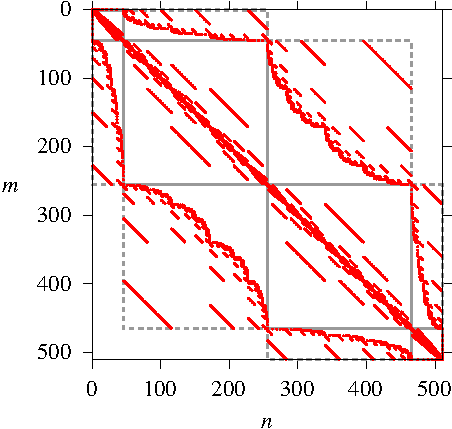
\includegraphics[width=0.45\textwidth]{04-Includes/Figures/matElem/matrixElements.pdf}
    \caption[Niezerowe elementy hamiltonianu]{Niezerowe elementy macierzowe $\qstatet{n}\hatH_{\text{Kitaev}+V}\qstate m$. ($\sites=10$, sektor parzysty, jednowymiarowy drut, \acrshort{OBC})}
    \label{fig:matElem}
\end{figure}

Na rysunku~\ref{fig:matElem} przedstawiono niezerowe elementy macierzowe hamiltonianu $\hatH_{\text{Kitaev}+V}$.
W tym przykładzie wyświetlono elementy macierzowe dla odpowiadającego układu o geometrii jednowymiarowego drutu $\sites=10$ (połączenia są tylko pomiędzy najbliższymi sąsiednimi węzłami $(i,j) \to (i,i+1)$), otwartych warunkach brzegowych \acrshort{OBC} oraz wybrano podprzestrzeń o parzystej liczbie cząstek.
Analogicznie jak na rysunku~\ref{fig:matrixElementConstruction}, na rysunku~\ref{fig:matElem} szarymi prostokątami zaznaczono odpowiednie sektory.


Większość programów, które pozwalają odtworzyć wyniki zamieszczone w tej pracy doktorskiej, można znaleźć w autorskiej bibliotece \href{https://github.com/andywiecko/SOLIDstate}{\texttt{\normalsize SOLIDstate}} napisanej w języku \texttt{\normalsize C++}, udostępnionej w serwisie \texttt{\normalsize github} (\texttt{\small https://github.com/andywiecko/SOLIDstate}) na licencji \texttt{\normalsize GPL}.
Biblioteka bazuje na potężnej bibliotece \href{http://arma.sourceforge.net/}{\arma}~\cite{sanderson.curtin.2016,sanderson.curtin.2019}.
\arma\ to tzw. \href{https://en.wikipedia.org/wiki/Wrapper_library}{\textit{wrapper}}, który może być interfejsem dla różnych bibliotek do algebry liniowej, takich jak \texttt{\normalsize LAPACK}, \texttt{\normalsize OPENBLAS}, \texttt{\normalsize ARPACK}, \texttt{\normalsize SUPERLU}, itd. %\linebreak
\arma\ posiada bardzo dobry balans pomiędzy szybkością wykonywania programów, a~łatwością obsługi ze względu na bardzo podobną składnię do wysokopoziomowego\linebreak \texttt{\normalsize MATLABa}.
\arma\ posiada klasy do przechowywania macierzy gęstych oraz rzadkich dla różnych danych, m.in. \texttt{\normalsize double}, \texttt{\normalsize complex<double>}, itd.
Biblioteka umożliwia rozwiązywanie równań Schr\"odingera (\acrshort{TISE}) takich jak równanie~\eqref{eq:eigenEquation} zarówno dla macierzy gęstych, jak i rzadkich.
Procedury dla macierzy gęstych korzystają z procedur dostępnych w \texttt{\normalsize LAPACK} [\glslink{ED}{dokładna diagonalizacja, (ED, ang. exact diagonalization)}], a procedury dla macierzy rzadkich korzystają z tych dostępnych na \texttt{\normalsize ARPACK}.
Te drugie bazują na algorytmie bazującym na przestrzeni Krylowa~\cite{krylov.1931} -- \acrfull{IRAM}~\cite{lehoucq.sorosen.1996}.
W~większości przypadków, struktura elementów macierzowych hamiltonianów w układach silnie skorelowanych jest bardzo rzadka.
Naturalne jest zatem przechowywanie danych w~postaci macierzy rzadkiej. 
W ten sposób można zyskać ogromne ilości pamięci operacyjnej komputerów.
Zarówno \acrshort{ED} jak i \acrshort{IRAM} mają swoje wady i zalety.
Zasadniczą zaletą metody \acrshort{ED} jest możliwość badania całego spektrum hamiltonianu.
W przypadku \acrshort{IRAM} ograniczenie jest do kilku wybranych wartości z~widma hamiltonianu.
Złożoność pamięciowa \acrshort{ED} wynosi $\bigO[(\dim\hilbertSpace)^2]$, a dla \acrshort{IRAM} zależy od układu. 
Dla typowych układów z fizyki silnie skorelowanych fermionów, ta zależność wynosi $\bigO(\dim\hilbertSpace)$.

\ornament